\documentclass[11pt,a4paper]{article}
\usepackage[margin=25mm]{geometry}
\usepackage{iftex}
\ifPDFTeX\usepackage[T1]{fontenc}\usepackage[utf8]{inputenc}\fi
\usepackage{amsmath,amssymb,graphicx,booktabs,array}
\usepackage[authoryear,round]{natbib}
\usepackage{caption,placeins}
\usepackage[unicode,breaklinks=true,hidelinks]{hyperref}
\setlength{\parindent}{0pt}\setlength{\parskip}{5pt}
\setlength{\emergencystretch}{3em}\setlength{\tabcolsep}{3pt}
\clubpenalty=10000\widowpenalty=10000
\captionsetup{font=small,labelfont=bf}
\newcounter{proposition}
\begin{document}
\begin{center}\Large\bfseries Hard to Beat: Historical Rules versus Conditional Quantile Models for Peak Net-Position Limits\end{center}

\begin{abstract}Dealers set limits on the largest position reached before a review horizon ends. Using hourly FX and weekly dealer positions, we compare conditional quantile forecasts with historical rules at matched history lengths and update schedules. Historical rules are demanding benchmarks. Long-history FX regression lowers matched loss by 14.8\% and 16.6\% in two periods. A calibration adjustment that updates after outcomes are observed retains the later gain (15.0\%), with 329 versus 328 breaches. Ranking against a shorter-history rolling rule changes across periods. On weekly aggregates, expanded regularization still leaves regression behind in 34 of 48 panel comparisons. Conservative short-sample validation also leaves large weekly losses. Lower scores accompany more breaches before calibration: 376 versus 360 in the matched FX comparison. These findings support selecting peak limits from accuracy, breaches and ranking stability together.\end{abstract}

\noindent\textbf{Keywords:} Peak net positions; Quantile forecasting; Historical benchmarks; Forecast comparison; Calibration; Dealer positions.\par\medskip

\section{Introduction}\label{sec:intro}

Dealer position limits concern the largest exposure reached before a review horizon ends. A position can finish within its limit after crossing it earlier (Figure~\ref{fig:example}). We compare historical and conditional forecasts of this sampled absolute-position peak.


Historical headroom already combines the current position with completed past peak behavior. Conditional models estimate additional relationships from finite historical windows. Matched histories and update schedules show whether the added conditioning improves the forecast.


\begin{figure}[htbp]\centering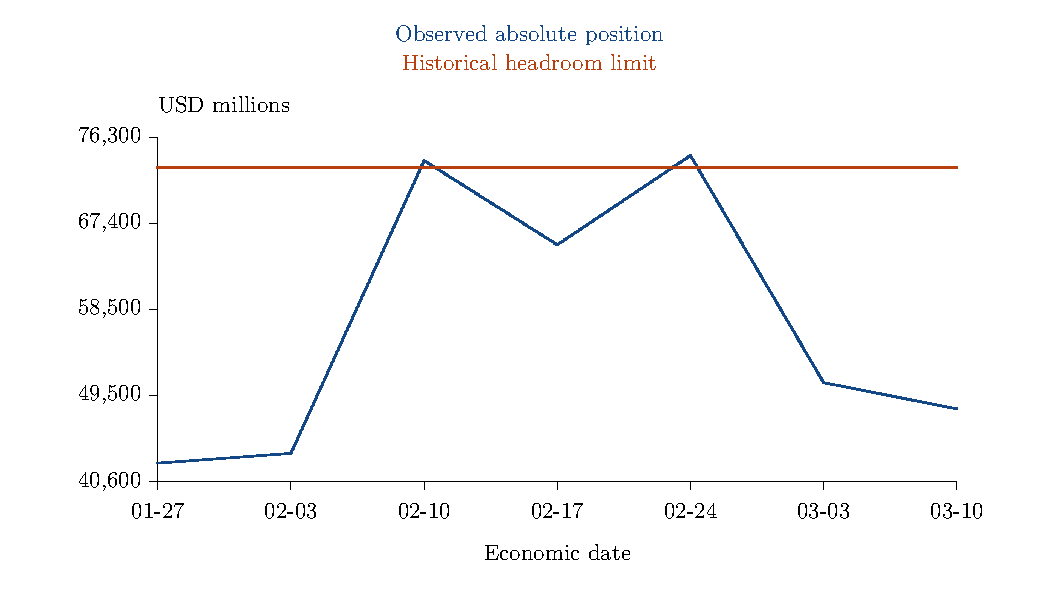
\includegraphics[width=.94\linewidth]{figures/v8-endpoint-peak-example.pdf}
\caption{An intervening Treasury-bill peak breaches the historical report although the endpoint lies inside it. The selected window is the earliest eligible original evaluation window.}\label{fig:example}
\end{figure}

Our comparisons cover hourly FX positions and weekly U.S. primary-dealer aggregates. Each series retains source-native units and its own evaluation grid. Two comparisons, pre-specified in the original execution protocol, anchor the analysis. They compare long-history FX regression with a shorter rolling rule, and Treasury regression with matched historical headroom.








The paper makes three empirical points.

\textit{First, matched FX gains recur across periods, and the later gain survives delayed calibration.} Regression lowers matched loss by 14.8\% and 16.6\% in the later and earlier periods (Table~\ref{tab:fx}). Calibration retains a 15.0\% gain with 329 versus 328 breaches. The shorter-history rolling reference reverses the earlier-period ranking.

\textit{Second, historical rules prevail across the weekly aggregate comparisons.} The Treasury-bill regression raises loss by 50.8\%, and expanded-menu regression still loses 34 of 48 additional-panel comparisons (Table~\ref{tab:weekly}). Conservative one-standard-error selection also leaves a worst-cell loss increase of 181.4\% in the earlier weekly period. More regularization and conservative validation therefore leave substantial observed gaps.

\textit{Third, lower quantile loss can coincide with more limit breaches.} The unwrapped matched FX gain comes with 376 versus 360 breaches (Table~\ref{tab:fx}). Elementary-score curves cross for both original main comparisons (Figures~\ref{fig:murphyfx} and~\ref{fig:murphybill}). Scores, error amounts and breach counts therefore provide complementary evidence for selecting a peak limit.

Section~\ref{sec:target} defines the target and records two elementary properties used later. The classical endpoint-to-peak bound supplies a separate benchmark under its stated assumptions. The subsequent sections compare matched forecasts, their stability and their implications for monitoring limits.

\FloatBarrier

\section{Related literature}\label{sec:literature}

Wisniewski and colleagues forecast signed next-hour position intervals using historical states, calendar information and local prediction methods \citep{wisniewski2020,wisniewski2024}. Their chronological training, calibration and test design reports scores and coverage together. The present peak response uses a complete future path segment and the current magnitude, producing different labels and limits.


Path-risk forecasts address within-period extremes. MaxVaR studies the worst cumulative portfolio return under fixed holdings and diffusion assumptions \citep{boudoukh2004}. The payment-liquidity thesis forecasts conditional maximum deficits from confidential transactions \citep{hoogen2017}. Settlement studies examine tail liquidity needs and collateral requirements \citep{petrunia2019,arjani2020}. Duffie and colleagues study dealer capacity and Treasury-market functioning, including PnL quantile forecasts \citep{duffie2023}. These responses differ from the sampled absolute-position peak.


Regression quantiles target asymmetric forecast errors directly \citep{koenker1978}. Autoregressive quantiles and quantile forests supply other conditioning structures \citep{engle2004,meinshausen2006}. Consistent scores and elementary-score representations permit comparison across evaluation preferences \citep{gneiting2011,ehm2016}. Table~\ref{tab:literature} locates the present peak response, completed labels and matched historical controls.


\begin{table}[htbp]\centering\footnotesize\uchyph=1\hyphenation{con-fi-den-tial con-di-tion-al re-gres-sion com-plet-ed el-e-men-ta-ry ex-pand-ing}
\caption{Closest literature and the peak-position task. A dash denotes a dimension unverified in the consulted passage. This study compares scores, breaches and reference stability for a common peak response.}\label{tab:literature}
\begin{tabular}{>{\raggedright\arraybackslash}p{2.4cm}>{\raggedright\arraybackslash}p{2.1cm}>{\raggedright\arraybackslash}p{1.5cm}>{\raggedright\arraybackslash}p{1.6cm}>{\raggedright\arraybackslash}p{1.6cm}>{\raggedright\arraybackslash}p{1.7cm}>{\raggedright\arraybackslash}p{1.7cm}}\toprule
Study & Response & Data unit & Peak floor & Label timing & Evaluation & Source scope\\\midrule
\shortstack[l]{Wisniewski\\et al. (2020)} & Signed endpoint interval & One FX market maker & --- & Ordered train/\allowbreak calibrate/\allowbreak test & Scores and hit tests & One source family\\
\shortstack[l]{Boudoukh\\et al. (2004)} & Worst portfolio return & Stylized fixed portfolio & Different initial-value anchor & Analytic diffusion & Tail ratios and monitoring & Parameter cases\\
\shortstack[l]{van den\\Hoogen (2017)} & Cumulative payment-deficit peak & Con\-fi\-den\-tial bank payments & --- & Path simulation & EVT methodology; results partly confidential & Bank payment task\\
\shortstack[l]{Duffie\\et al. (2023)} & Capacity, illiquidity, PnL quantiles & Dealer/\allowbreak market sources & --- & Expanding PnL fits & Capacity and PnL forecasts & Several sources\\
\shortstack[l]{Engle and\\Manganelli\\(2004)} & Return quantile & Asset returns & --- & Lagged predictors & Quantile scores and DQ & Several returns\\
\shortstack[l]{Ehm et al.\\(2016)} & Quantile/\allowbreak expectile comparison & Multiple forecast examples & --- & Original example designs & El\-e\-men\-tary-score curves & Multiple tasks\\
\shortstack[l]{Meinshausen\\(2006)} & Conditional response quantile & Regression examples & --- & Original regression splits & Conditional distributions & Several datasets\\
This study & Sampled absolute-position peak & One FX record; weekly totals & Observed current magnitude & Completed forward labels & Scores, breaches, coherence & Related aggregate tasks\\
\bottomrule\end{tabular}
\par\smallskip\begin{minipage}{.98\linewidth}\footnotesize The payment-thesis reading is partial. Dashes identify unverified dimensions in the consulted passages.\end{minipage}
\end{table}

First, matched FX gains recur (14.8\%, 16.6\%), and the later gain survives calibration; rolling-reference rankings change (Table~\ref{tab:fx}). Second, expanded weekly regression loses 34 of 48 comparisons; conservative selection leaves a 181.4\% worst excess (Table~\ref{tab:weekly}). Third, matched FX gains coincide with 376 versus 360 breaches, and the original elementary-score curves cross (Table~\ref{tab:diagnostics}; Figures~\ref{fig:murphyfx}--\ref{fig:murphybill}).

\FloatBarrier

\section{The forecast target}\label{sec:target}

The target is the largest sampled absolute position from issue time through the stated horizon. Let \(N_t\) denote signed position and \(\mathcal F_t\) the issue-time information. The peak \(Y_{t,H}\), observed floor \(B_t\) and nonnegative headroom \(Z_{t,H}\) satisfy the following identities.


\[
Y_{t,H}=\max_{0\le h\le H}|N_{t+h}|,\qquad B_t=|N_t|,\qquad Z_{t,H}=Y_{t,H}-B_t\ge0.
\]

A feasible limit covers the current observed exposure. Figure~\ref{fig:example} shows an endpoint inside the historical report after an earlier breach. We score reports with pinball loss and count a strict breach when the peak exceeds the limit.


\[
\rho_\tau(u)=\tau u_+ +(1-\tau)(-u)_+,\qquad I_{t,H}=\mathbf 1\{Y_{t,H}>C_{t,H}\}.
\]

\refstepcounter{proposition}\noindent\textbf{Proposition~\theproposition (known-floor projection).}\label{prop:floor} Suppose \(Y\ge B\) almost surely and the issue information contains \(B\). Projecting any forecast \(c\) to \(\max\{B,c\}\) weakly improves pinball loss for every possible outcome, with an exact gain below the floor. If \(q\) is the true conditional lower inverse quantile at level \(1-\alpha\), its strict exceedance probability is at most \(\alpha\). At an atom of the response distribution, that probability can be smaller than the nominal tail probability.


\[
\rho_\tau(Y-c)-\rho_\tau(Y-\max\{B,c\})=\tau(B-c)_+,\qquad \Pr(Y>q\mid\mathcal F_t)\le\alpha.
\]

\refstepcounter{proposition}\noindent\textbf{Proposition~\theproposition (classical endpoint-to-peak bound).}\label{prop:levy} Let future increments be independent and individually symmetric about zero, with partial sums \(S_h\). Fix a starting position \(x\), set \(B=|x|\), and let \(q\) be the population \((1-\alpha/2)\) quantile of \(|S_H|\). The triangle inequality and the classical scalar L\'evy maximal inequality then imply the following bound, including strict inequalities at atoms \citep{sussman2023}. Neither identical increment distributions nor finite increment moments are required for this population statement.


\[
\Pr\!\left(\max_{0\le h\le H}|x+S_h|>B+q\right)\le\Pr\!\left(\max_h|S_h|>q\right)\le2\Pr(|S_H|>q)\le\alpha.
\]

The Supplement proves both statements and compares population quantiles with their empirical plug-ins. A conditional application requires independence, symmetry and the stated endpoint quantile under the law given issue information. The separate bound simulations distinguish mean-reverting levels from serially correlated increments.


Separately fitted horizon forecasts can violate the ordering of true peak quantiles. Short-history FX regression crosses across horizons on 640 evaluation origins. Label nesting, floor coverage and strict-breach definitions provide additional checks on the issued reports.


\FloatBarrier

\section{Data}\label{sec:data}

The FX application uses the hourly Net Position Time Series Dataset, reporting market-maker client-flow positions \citep{dataset,wisniewski2020}. It contains 18,576 observation records in source USD units. The later and earlier comparisons use distinct chronological issue grids and the same sampled-peak definition.


The weekly data are New York Fed Primary Dealer Statistics \citep{nyfeddata}. Reporting definitions follow the government-securities dealer framework and position-accounting instructions \citep{fr2004_2013,fr2004_2024}. The Treasury-bill series has 706 economic-date observations in USD millions. These are reported fair-value positions aggregated as long-minus-short totals. Additional categories pass metadata and calendar checks and use complete weekly grids, with separate fits by category.


Every method within a comparison uses identical peak labels, current floors and issue origins. Source units and histories remain distinct across series. This design preserves the measurement differences between FX client flow and weekly position totals.


\FloatBarrier

\section{Forecasting methods}\label{sec:methods}

Forecasts target the conditional quantile at \(\tau=19/20\). The horizons \(H\in\{6,24\}\) count subsequent source records, and each peak includes the issue position. Calendar gaps extend the elapsed span of an FX horizon, while weekly steps represent a different review interval. All methods forecast this common target.


Historical headroom uses the corrected empirical rank of completed headrooms and adds its report to the current magnitude. Translated paths reanchor historical signed paths, while historical-peak quantiles are projected to the observed floor. The endpoint plug-in uses an absolute-displacement quantile; Table~\ref{tab:methods} gives the executed menus and schedules.


Ridge quantile regression links mature headroom to issue-known position states and calendar variables. The larger set contains 33 predictors plus an unpenalized intercept. The four-predictor variant uses current magnitude, signed level and two increment RMS measures. All standardization uses mature training observations. Expanded-menu regression changes only the penalty grid.


Local quantiles use neighboring historical states, with an increment-scaled variant. Filtered paths simulate positions from GARCH-standardized empirical innovations drawn independently with replacement \citep{hull1998,barone1999}. Quantile forests use leaf distributions; tail methods fit volatility-scaled headroom \citep{meinshausen2006,mcneilfrey2000}. The Supplement lists all complete results and numerical or structural failures.


Additional comparisons apply delayed calibration, fixed combinations and conservative selection to the same peak response. A headroom CAViaR recursion and calibration wrappers follow existing methods \citep{engle2004,gibbs2021}. Calibration parameters update after outcomes mature. Fixed mean and median combinations use predefined members. Conservative selection favors the strongest shrinkage whose paired mean-loss excess against the validation winner falls within one heteroskedasticity and autocorrelation consistent (HAC) standard error.


\begin{table}[htbp]\centering\small
\caption{Historical and conditional forecasts use a common completed-peak response; menus and schedules are the executed settings.}\label{tab:methods}
\begin{tabular}{>{\raggedright\arraybackslash}p{2.9cm}>{\raggedright\arraybackslash}p{6.0cm}>{\raggedright\arraybackslash}p{5.3cm}}\toprule
Method / code & Forecast definition & Executed menu / setting\\\midrule
Historical headroom (F) & Current floor plus a quantile of completed peak headrooms & FX histories \{720,2880\}; weekly \{52,260\}\\
Translated path (S) & Translate completed signed paths to the current position before taking their peaks & Same completed-label pools; fixed-window and rolling-window controls\\
Historical peak (K) & Historical absolute-peak quantile projected to the current floor & Same histories and update controls\\
Quantile regression (QR) & Training-scaled headroom regression with ridge slopes and an unpenalized intercept & Original penalties $\{0.001,0.01,0.1\}$; expanded menu in Supplement\\
Local quantiles (KNN) & Neighbor headroom quantile, with a separate increment-scale variant & Training-only transforms and fixed neighbor menus; Supplement\\
Parsimonious regression (QR4) & Current signed/magnitude positions and short/long increment RMS & Separate five-point penalty menu; common-menu comparison in Supplement\\
Endpoint plug-in (L) & Floor plus a high absolute-displacement endpoint quantile & Proposition~\ref{prop:levy}; empirical plug-in evaluated separately\\
Further benchmarks & Autoregressive replay; filtered paths; peak-tail fit; quantile forest & Existing bounded specifications, complete failures included in Supplement\\
Coverage and combinations & Delayed projected ACI-style wrappers; headroom SAV; fixed forecast combinations & Original-source wrapper/SAV inventory and broader combination inventory are separate\\
\bottomrule\end{tabular}
\par\smallskip\begin{minipage}{.98\linewidth}\footnotesize Training histories count completed labels. Fixed-window models refit every 24 FX records or 13 weekly records. The Supplement specifies quantile and normalization conventions.\end{minipage}
\end{table}

\FloatBarrier

\section{Evaluation design}\label{sec:evaluation}

At refit \(r\), training labels are eligible only when \(i+H\le r\). Predictors use issue-known observations, and training transforms remain fixed until the next refit. The preceding validation segment selects parameters; the entire specified evaluation grid then receives forecasts. Weekly selection uses 52 outer validation origins with overlapping labels.


Matched comparisons fix completed-response history and refit schedule for regression and historical headroom. The main FX reference uses a shorter rolling history; the main Treasury reference shares regression's longer history and refit schedule. Tables~\ref{tab:fx} and~\ref{tab:weekly} report both alongside the other comparison sets.


Accuracy uses mean pinball loss; breaches are strict peak exceedances. Evaluation scores passive reports on the observed position paths. Paired loss differences use HAC covariance with the horizon-based bandwidth rule \citep{dm1995,nw1987}. Tables report the small-sample adjustment and named multiplicity families \citep{hln1997,holm1979}. Coverage diagnostics use the fixed spaced grid and condition the transition likelihood on its initial hit \citep{kupiec1995,christ1998}.


\subsection{Research design and transparency}

The original protocol fixes the two main comparisons and their reference procedures. Other p-values are exploratory and unadjusted unless stated. The Supplement records chronology, comparison families and all failure inventories.





\FloatBarrier

\section{Results}\label{sec:results}

\subsection{Where conditional models improve}

Long-history FX regression beats matched historical headroom in both periods. Loss falls by 14.8\% later and 16.6\% earlier. Table~\ref{tab:fx} separates these matched controls from the shorter rolling reference.


Delayed calibration retains the later matched FX gain. Wrapped regression lowers loss by 15.0\%. Its 329 breaches compare with 328 for wrapped historical headroom on common origins (Table~\ref{tab:fx}).


The long-history FX gain persists across training-defined increment-RMS states and at the lower target quantile. At the lower target, matched loss falls by 10.1\%, and loss against the original rolling reference by 9.2\%. The Supplement reports all state results and failed validation at the upper quantile.


\begin{table}[htbp]\centering\small
\caption{Long-history short-horizon FX regression under two references and periods. Negative percentages favor regression. Matched gains recur while the rolling-reference direction changes.}\label{tab:fx}
\begin{tabular}{>{\raggedright\arraybackslash}p{2.6cm}>{\raggedright\arraybackslash}p{4.4cm}>{\raggedright\arraybackslash}p{2.5cm}>{\raggedright\arraybackslash}p{1.5cm}>{\raggedright\arraybackslash}p{3.2cm}}\toprule
Period / procedure & Reference & Loss change (\%) & Issues & Strict breaches (regression / reference)\\\midrule
Later / main comparison & Shorter-history rolling headroom & -12.7 & 6625 & 376 / 332\\
Later / matched & Same-history fixed-window headroom & -14.8 & 6625 & 376 / 360\\
Earlier / original structure & Shorter-history rolling headroom & +3.2 & 1440 & See complete earlier-period tables\\
Earlier / matched & Same-history fixed-window headroom & -16.6 & 1440 & 20 / 16\\
Later / coverage-wrapped & Same-history wrapped headroom & -15.0 & 6625 & 329 / 328\\
\bottomrule\end{tabular}
\par\smallskip\begin{minipage}{.98\linewidth}\footnotesize Regression uses history 2880 and horizon 6; the original rolling reference uses 720. The earlier matched comparison is the original three-penalty regression, not the later one-standard-error selection rule. The wrapper comparison is a separate finite projected delayed ACI-style exercise; both regression and historical headroom are calibrated in that row.\end{minipage}
\end{table}

\subsection{Where conditional models lose}

The earlier FX ranking reverses when the reference changes. Against shorter-history rolling headroom, later loss falls by 12.7\%, but earlier loss rises by 3.2\%. Matched gains and rolling-reference gains therefore have different period stability (Table~\ref{tab:fx}).


Short-history FX regression performs poorly at the longer horizon. Loss rises by 31.5\% against matched historical headroom. Regression records 924 breaches against 427 for the reference; the full horizon map retains the other adverse comparisons.


Treasury-bill regression loses on both accuracy and breaches. Mean loss rises by 50.8\%, with 54 regression breaches. Historical headroom records 28 breaches; the earlier short-window version also loses (Table~\ref{tab:weekly}).


Stronger regularization narrows weekly panel losses but leaves historical rules ahead. Median excess loss falls from 92.6\% to 9.2\% after menu expansion. Regression still loses 34 of 48 matched comparisons. In the earlier weekly grid, conservative selection's worst increase is 181.4\%. The adverse cell is the Treasury-bill short-window, 24-step comparison (Table~\ref{tab:weekly}).


Simpler conditional reports and fixed combinations also give mixed weekly results. The median combination lowers Treasury-bill loss by 4.0\%, while the mean combination raises it by 2.8\%. The headroom recursion is also worse; Table~\ref{tab:weekly} and the Supplement retain every completed loss and model failure.


\begin{table}[htbp]\centering\small
\caption{Weekly loss changes for distinct history and selection settings. Expanding the penalty menu reduces losses while leaving historical headroom ahead in most panel cells.}\label{tab:weekly}
\begin{tabular}{>{\raggedright\arraybackslash}p{4.3cm}>{\raggedright\arraybackslash}p{4.7cm}>{\raggedright\arraybackslash}p{2.7cm}>{\raggedright\arraybackslash}p{2.5cm}}\toprule
Comparison set & Procedure & Loss change / median (\%) & Higher-loss cells\\\midrule
Treasury-bill main comparison & Original regression, long history & +50.8 & Main comparison\\
Earlier Treasury-bill short window & Short-history regression & +144.3 & Different history\\
Additional panel & Original full regression & +92.6 & 45 / 48\\
Additional panel & Four-predictor regression & +9.9 & 37 / 48\\
Additional panel & Full regression, expanded penalties & +9.2 & 34 / 48\\
Additional panel & Ordinary empirical headroom quantile & +0.5 & 30 / 48\\
Earlier weekly groups & Validation-minimum expanded rule & +4.2 & 26 groups\\
Earlier weekly groups & One-standard-error rule & +5.4 & 26 groups\\
\bottomrule\end{tabular}
\par\smallskip\begin{minipage}{.98\linewidth}\footnotesize The bill main comparison has 54 versus 28 strict breaches among 277 issues; earlier weekly cells each have 52 evaluation points. The earlier bill comparison uses history 52 instead of 260; its conservative-selection worst cell is the 24-step bill case (181.4\%). All three preset success criteria remain unmet.\end{minipage}
\end{table}

\subsection{Scores and breach behavior answer different questions}

Lower FX loss coexists with more breaches before calibration. Regression breaches 376 times against 360 for matched historical headroom. Pinball loss measures error amounts, while a strict-hit indicator records event occurrence; both matter for choosing monitoring limits.


Elementary-score rankings cross for both main comparisons (Figures~\ref{fig:murphyfx} and~\ref{fig:murphybill}). A separate 24-step FX comparison against rolling translated paths reverses near 20.6:1. Both six-step FX comparisons improve mean overrun and unused allowance, so that weight reversal belongs to the 24-step reference.


Loss and coverage tests answer different questions (Table~\ref{tab:diagnostics}). HAC tests compare average loss; strict-hit tests examine event frequency and serial behavior. RMS-state diagnostics compare conditional predictive ability across training-defined groups \citep{gw2006}.


\begin{table}[htbp]\centering\small
\caption{Paired loss tests and strict-hit diagnostics for the explicitly named reports. Panel A uses working-reference inference; Panel B uses the fixed nonoverlap grid.}\label{tab:diagnostics}
\begin{tabular}{>{\raggedright\arraybackslash}p{4.3cm}>{\raggedright\arraybackslash}p{2.1cm}>{\raggedright\arraybackslash}p{2.1cm}>{\raggedright\arraybackslash}p{5.7cm}}\toprule
Panel A: paired contrast & DM p & HLN p & Named adjustment / p\\\midrule
FX main comparison & 2.2e-07 & 2.31e-07 & Bonferroni (two main comparisons): 4.39e-07\\
FX matched history & 4.47e-09 & 4.83e-09 & Original matched Holm family: 2.86e-07\\
Treasury main comparison & 0.00761 & 0.00939 & Original matched Holm family: 0.32\\
\bottomrule\end{tabular}
\par\smallskip\begin{minipage}{.98\linewidth}\footnotesize Original matched Holm uses 72 contrasts. Each adjusted p-value applies only to its named family; the later regrouped family is separate.\end{minipage}

\par\medskip\begin{center}\small
\begin{tabular}{p{4.0cm}rrrr}\toprule
Panel B: report & Grid hits & Grid issues & Kupiec p & Christoffersen CC p\\\midrule
FX regression & 50 & 947 & 0.695 & 0.636\\
FX original rolling reference & 49 & 947 & 0.807 & 0.905\\
FX matched fixed reference & 49 & 947 & 0.807 & 0.646\\
Treasury regression & 7 & 40 & 0.00413 & 0.0136\\
Treasury historical reference & 4 & 40 & 0.199 & 0.262\\
\bottomrule\end{tabular}\end{center}
{\footnotesize Hit tests use the full fixed nonoverlap grid; the conditional-coverage likelihood conditions on its initial hit. Equality to the nominal tail rate is the stated diagnostic null, distinct from the population upper-quantile inequality. The grid does not create independence.}
\end{table}

\begin{figure}[htbp]\centering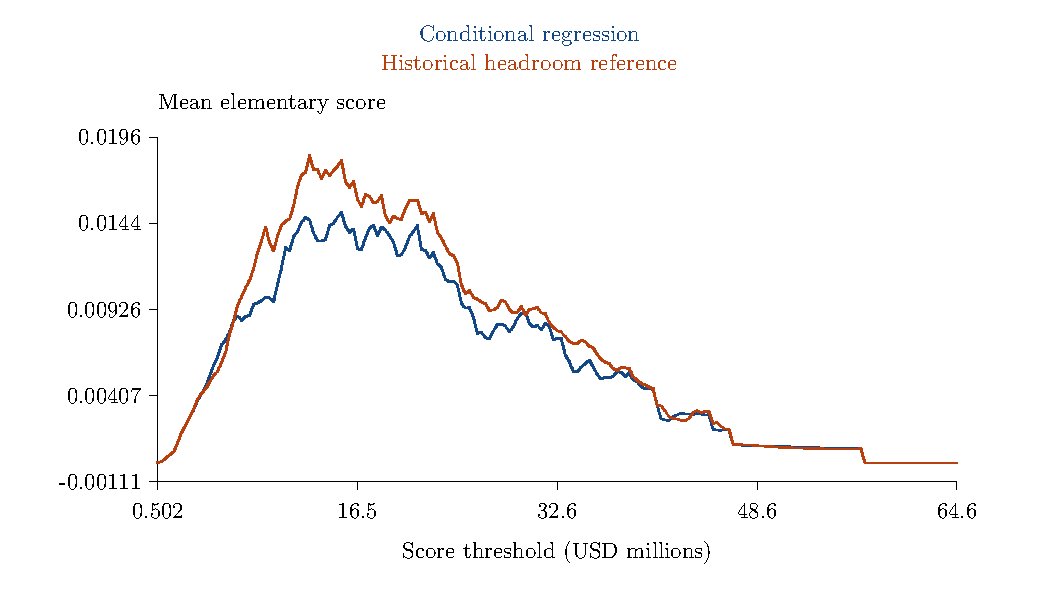
\includegraphics[width=.94\linewidth]{figures/v7-murphy-fx_hourly.pdf}
\caption{Crossing elementary-score curves for the FX main comparison against rolling headroom. Curves use a display grid; full-breakpoint comparisons confirm crossings.}\label{fig:murphyfx}
\end{figure}

\begin{figure}[htbp]\centering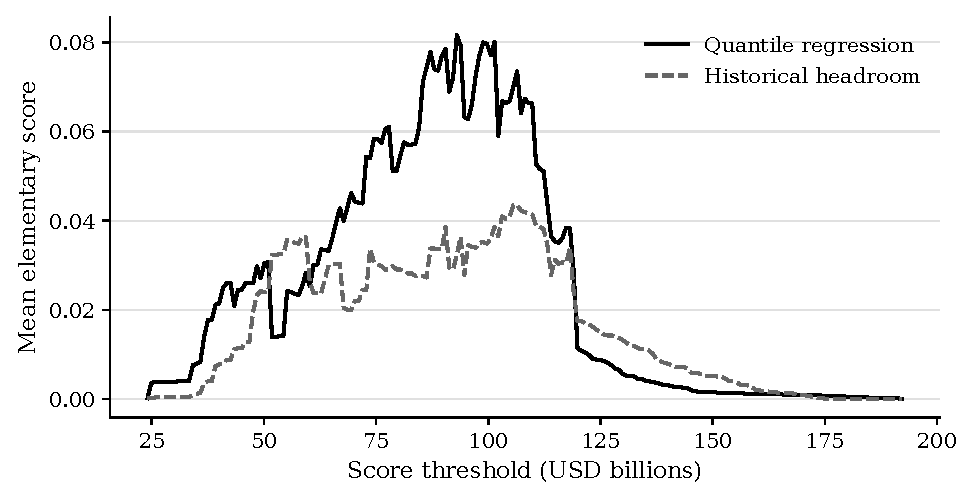
\includegraphics[width=.94\linewidth]{figures/v7-murphy-nyfed_weekly.pdf}
\caption{Elementary-score curves cross for the Treasury-bill main comparison. Curves use a display grid; full-breakpoint comparisons confirm crossings.}\label{fig:murphybill}
\end{figure}

\FloatBarrier


\subsection{Why historical rules are hard to beat: a calibrated simulation}\label{sec:calibrated-mc}

The calibrated simulation does not reproduce the persistent weekly losses in the financial record. Weekly GARCH median loss changes from +0.4\% to -20.6\% (Figure~\ref{fig:calibrated-mc}). This comparison uses 33 predictors and histories of 52 and 2880 completed responses. The constant-variance AR process also retains useful level-state information. Seven of eight hourly cells fail numerical acceptance; each entire cell is reported failed. Prespecified predictions of at most 2.0\% gain under constant variance and over 5.0\% loss in short weekly samples are unsupported; hourly failures preclude assessment of long-history gains and the joint trend (Supplement Table~S32).

\begin{figure}[htbp]\centering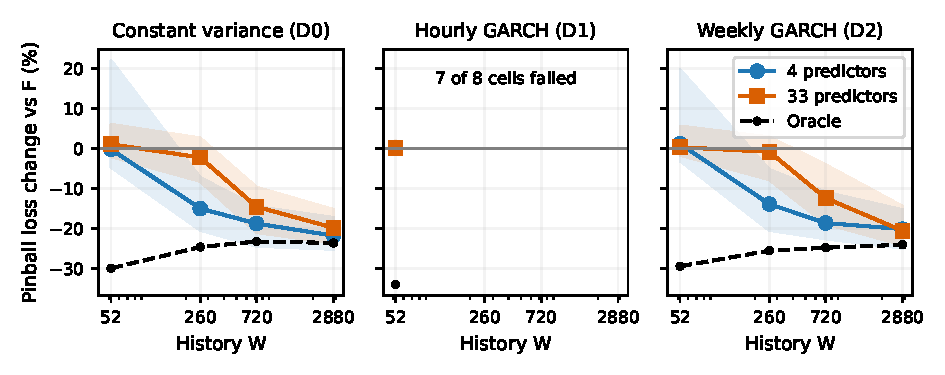
\includegraphics[width=.98\linewidth]{figures/v8-calibrated-mc.pdf}
\caption{Calibrated simulation: median regression loss changes against F, with IQRs shaded. Each complete cell uses 100 repetitions of 500 origins; dashed curves and black dots are finite oracles from 2,000 future paths per origin. Seven hourly cells failed; the Supplement's calibrated-simulation section gives full setting details.}\label{fig:calibrated-mc}
\end{figure}

\FloatBarrier

\section{Implications for model validation}\label{sec:implications}

\textbf{Benchmark against historical headroom.} Use the same completed labels, history length and refit schedule. The FX ranking against shorter rolling history changes across periods, showing why the control must be named.


\textbf{In short weekly samples, default to the corrected-rank historical rule.} Expanded regularization and conservative one-standard-error selection leave large observed losses. The ordinary empirical quantile is up to 36.5\% worse than corrected F in the earlier weekly grid. Change to a conditional report when validation across periods and controls supports the decision.


\textbf{Report breaches with the score.} Show mean underprediction, mean unused headroom and strict-breach count on the same grid. The matched unwrapped FX gain records 376 versus 360 breaches; Table~\ref{tab:map} summarizes the validation decisions.


\begin{table}[htbp]\centering\small
\caption{Financial and stationary-simulation findings for the specified histories and horizons. The action column states how each comparison informs peak-limit validation.}\label{tab:map}
\begin{tabular}{>{\raggedright\arraybackslash}p{2.7cm}>{\raggedright\arraybackslash}p{3.8cm}>{\raggedright\arraybackslash}p{4.0cm}>{\raggedright\arraybackslash}p{3.2cm}}\toprule
Setting & Financial evidence & Simulation support & Validation action\\\midrule
Hourly / long history / short horizon & Repeated matched gains; separate wrapper check & Unresolved: corresponding hourly cells fail & Compare named control and breaches\\
Hourly / short history / short horizon & Small score gain with more breaches & Unresolved at the financial history length & Require stable joint performance\\
Hourly / either history / longer horizon & Losses or weaker gains; preference sensitivity & Not simulated at the longer horizon & Check horizon order and loss preferences\\
Weekly / either history / either horizon & Frequent losses despite expanded penalties & Short-horizon losses not reproduced; longer horizon untested & Retain historical and parsimonious controls\\
Endpoint bound / specified horizon & Population premises and plug-in behavior differ & Separate bound simulation in Supplement; not this calibrated grid & Check displacement and dependence\\
\bottomrule\end{tabular}

\end{table}

\FloatBarrier

\section{Limitations}\label{sec:limitations}

The FX data describe a single market maker's client-flow record. Its original evaluation period was viewed before the conditional methods were specified. The earlier 2015 comparison was designed after the original results and is retrospective.


The weekly categories share a reporting system and economic components, so related series are not independent dealer replications. Treasury comparisons replay the downloaded economic-date vintage; historical publication-time information is not reconstructed. Aggregation can offset gross dealer exposure, and between-observation excursions remain unmeasured.


Causal and individual-predictor effects are outside this design. The financial procedures provide no coverage guarantee under their dependence and calibration scheme. Trading and funding gains are not measured, and scoring weights do not identify actual decision costs. Independent dealer data and prospective evaluation are needed for broader validation. Valuation, gross-exposure and decision-cost observations would connect forecasts to inventory actions.

The calibrated simulations leave the hourly mechanism unresolved and fail to reproduce persistent weekly losses. Their DGPs bundle frequency, validation length and volatility laws. Isolating these effects and studying failed hourly fits requires a separate experiment. Longer chronologically eligible validation histories also require future evaluation.


\FloatBarrier

\section{Conclusion}\label{sec:conclusion}

Simple historical rules are hard to beat for peak net positions in these records. FX regression lowers matched loss by 14.8\% and 16.6\% across periods. Calibration retains the later gain with 329 versus 328 breaches. The shorter rolling reference changes the earlier ranking.

Expanded regularization leaves weekly regression behind in 34 of 48 panel comparisons, and conservative validation leaves large losses. Lower FX pinball loss coexists with 376 versus 360 breaches before calibration. Peak-limit selection should assess accuracy, error amounts, breaches and reference stability together.

\FloatBarrier

\section*{Data and code availability}
\paragraph{Data availability.} The FX input is the specified version of the Kaggle Net Position Time Series Dataset. The owning metadata labels its license ``Data files \copyright\ Original Authors.'' This repository supplies the acquisition route and input fingerprint, but excludes raw FX observations and private per-issue prediction vectors. Obtain the source from \url{https://www.kaggle.com/datasets/davidlindsay1979/net-position-time-series-dataset} subject to the original rights holders' terms.

The New York Fed aggregates are available from its Primary Dealer Statistics service under the Bank's Terms of Use. The repository preserves the unchanged accepted Treasury snapshot with attribution and identifies study calculations separately. Copying or distributing that content remains subject to its source notices, attribution, modification labelling, continuing conditions and endorsement restrictions: \url{https://www.newyorkfed.org/privacy/termsofuse.html}. The code license does not replace those source conditions.

\paragraph{Code availability.} Code, saved financial results and calibrated-simulation outputs are available at \url{https://github.com/ByronLi0207/financial-mathematics-paper-20261020/tree/revision-v8}. The package README gives native document compilation; frozen protocols describe separate restricted-input replays. This revision adds no new financial forecast evaluation. The completed results include adverse, failed and unavailable cases.

\section*{Author-provided information}
Author information: [TO BE COMPLETED BY AUTHOR].\par
ORCID: [TO BE COMPLETED BY AUTHOR].\par
Funding: [TO BE COMPLETED BY AUTHOR].\par
Competing interests: [TO BE COMPLETED BY AUTHOR].\par
AI statement: [TO BE COMPLETED BY AUTHOR].

\begin{thebibliography}{99}
\bibitem[Arjani et al.(2020)]{arjani2020} Arjani, N., Li, F., \& Sabetti, L. (2020). \emph{Monitoring intraday liquidity risks in a real time gross settlement system}. Payments Canada. \url{https://www.payments.ca/sites/default/files/discussion_paper_monitoring_intraday_liquidity_risks_in_a_real_time_gross_settlement_system.pdf}.

\bibitem[Barone-Adesi et al.(1999)]{barone1999} Barone-Adesi, G., Giannopoulos, K., \& Vosper, L. (1999). VaR without correlations for portfolios of derivative securities. \emph{Journal of Futures Markets}, \emph{19}(5), 583--602. \url{https://doi.org/10.1002/(SICI)1096-9934(199908)19:5<583::AID-FUT5>3.0.CO;2-S}.

\bibitem[Board of Governors of the Federal Reserve System(2013)]{fr2004_2013} Board of Governors of the Federal Reserve System (2013, March). \emph{Reporting guidelines for preparing the FR 2004 primary government securities dealers reports}. Board of Governors of the Federal Reserve System. \url{https://www.federalreserve.gov/apps/reportingforms/Download/DownloadAttachment?guid=f555fe11-e149-479b-8088-4ed4e9ae1206}.

\bibitem[Board of Governors of the Federal Reserve System(2024)]{fr2004_2024} Board of Governors of the Federal Reserve System (2024, July). \emph{Instructions for the preparation of government securities dealers reports: Reporting form FR 2004}. Board of Governors of the Federal Reserve System. \url{https://www.federalreserve.gov/apps/reportingforms/Download/DownloadAttachment?guid=950ab256-b485-4586-99b0-b27eb205fdfa}.

\bibitem[Boudoukh et al.(2004)]{boudoukh2004} Boudoukh, J., Richardson, M., Stanton, R., \& Whitelaw, R. F. (2004). MaxVaR: Long-horizon value at risk in a mark-to-market environment. \emph{Journal of Investment Management}, \emph{2}(3), 1--6. \url{https://pages.stern.nyu.edu/~rwhitela/papers/maxvar%20joim04.pdf}.

\bibitem[Christoffersen(1998)]{christ1998} Christoffersen, P. F. (1998). Evaluating interval forecasts. \emph{International Economic Review}, \emph{39}(4), 841--862. \url{https://doi.org/10.2307/2527341}.

\bibitem[Diebold \& Mariano(1995)]{dm1995} Diebold, F. X., \& Mariano, R. S. (1995). Comparing predictive accuracy. \emph{Journal of Business \& Economic Statistics}, \emph{13}(3), 253--263. \url{https://doi.org/10.1080/07350015.1995.10524599}.

\bibitem[Duffie et al.(2023)]{duffie2023} Duffie, D., Fleming, M. J., Keane, F. M., Nelson, C., Shachar, O., \& Van Tassel, P. (2023). \emph{Dealer capacity and U.S. Treasury market functionality} (Staff Report No. 1070). Federal Reserve Bank of New York Staff Reports. \url{https://doi.org/10.59576/sr.1070}.

\bibitem[Ehm et al.(2016)]{ehm2016} Ehm, W., Gneiting, T., Jordan, A., \& Krüger, F. (2016). Of quantiles and expectiles: Consistent scoring functions, choquet representations and forecast rankings. \emph{Journal of the Royal Statistical Society Series B: Statistical Methodology}, \emph{78}(3), 505--562. \url{https://doi.org/10.1111/rssb.12154}.

\bibitem[Engle \& Manganelli(2004)]{engle2004} Engle, R. F., \& Manganelli, S. (2004). CAViaR: Conditional autoregressive value at risk by regression quantiles. \emph{Journal of Business \& Economic Statistics}, \emph{22}(4), 367--381. \url{https://doi.org/10.1198/073500104000000370}.

\bibitem[Federal Reserve Bank of New York(n.d.)]{nyfeddata} Federal Reserve Bank of New York (n.d.). \emph{Primary dealer statistics} [Data set]. Federal Reserve Bank of New York. \url{https://www.newyorkfed.org/markets/counterparties/primary-dealers-statistics}. Retrieved October 23, 2026.

\bibitem[Giacomini \& White(2006)]{gw2006} Giacomini, R., \& White, H. (2006). Tests of conditional predictive ability. \emph{Econometrica}, \emph{74}(6), 1545--1578. \url{https://doi.org/10.1111/j.1468-0262.2006.00718.x}.

\bibitem[Gibbs \& Candès(2021)]{gibbs2021} Gibbs, I., \& Candès, E. J. (2021). Adaptive conformal inference under distribution shift. \emph{Advances in Neural Information Processing Systems}, \emph{34}, 1660--1672. \url{https://proceedings.neurips.cc/paper_files/paper/2021/hash/0d441de75945e5acbc865406fc9a2559-Abstract.html}.

\bibitem[Gneiting(2011)]{gneiting2011} Gneiting, T. (2011). Making and evaluating point forecasts. \emph{Journal of the American Statistical Association}, \emph{106}(494), 746--762. \url{https://doi.org/10.1198/jasa.2011.r10138}.

\bibitem[Harvey et al.(1997)]{hln1997} Harvey, D., Leybourne, S., \& Newbold, P. (1997). Testing the equality of prediction mean squared errors. \emph{International Journal of Forecasting}, \emph{13}(2), 281--291. \url{https://doi.org/10.1016/s0169-2070(96)00719-4}.

\bibitem[Holm(1979)]{holm1979} Holm, S. (1979). A simple sequentially rejective multiple test procedure. \emph{Scandinavian Journal of Statistics}, \emph{6}(2), 65--70. \url{https://www.jstor.org/stable/4615733}.

\bibitem[Hull \& White(1998)]{hull1998} Hull, J., \& White, A. (1998). Incorporating volatility updating into the historical simulation method for value-at-risk. \emph{The Journal of Risk}, \emph{1}(1), 5--19. \url{https://doi.org/10.21314/jor.1998.001}.

\bibitem[Koenker \& Bassett(1978)]{koenker1978} Koenker, R., \& Bassett, G., Jr. (1978). Regression quantiles. \emph{Econometrica}, \emph{46}(1), 33--50. \url{https://doi.org/10.2307/1913643}.

\bibitem[Kupiec(1995)]{kupiec1995} Kupiec, P. H. (1995). Techniques for verifying the accuracy of risk measurement models. \emph{The Journal of Derivatives}, \emph{3}(2), 73--84. \url{https://doi.org/10.3905/jod.1995.407942}.

\bibitem[Lindsay(2020)]{dataset} Lindsay, D. (2020). \emph{Net position time series dataset} (Version 2) [Data set]. Kaggle. \url{https://www.kaggle.com/datasets/davidlindsay1979/net-position-time-series-dataset}.

\bibitem[McNeil \& Frey(2000)]{mcneilfrey2000} McNeil, A. J., \& Frey, R. (2000). Estimation of tail-related risk measures for heteroscedastic financial time series: An extreme value approach. \emph{Journal of Empirical Finance}, \emph{7}(3--4), 271--300. \url{https://doi.org/10.1016/s0927-5398(00)00012-8}.

\bibitem[Meinshausen(2006)]{meinshausen2006} Meinshausen, N. (2006). Quantile regression forests. \emph{Journal of Machine Learning Research}, \emph{7}(35), 983--999. \url{https://www.jmlr.org/papers/v7/meinshausen06a.html}.

\bibitem[Newey \& West(1987)]{nw1987} Newey, W. K., \& West, K. D. (1987). A simple, positive semi-definite, heteroskedasticity and autocorrelation consistent covariance matrix. \emph{Econometrica}, \emph{55}(3), 703--708. \url{https://doi.org/10.2307/1913610}.

\bibitem[Petrunia et al.(2019)]{petrunia2019} Petrunia, R., Sabetti, L., \& Voia, M. (2019). \emph{Tail risk in the automated clearing settlement system (ACSS)} (Discussion Paper No. 7). Payments Canada. \url{https://www.payments.ca/sites/default/files/tail_risk_in_the_automated_clearing_settlement_system_acss.pdf}.

\bibitem[Sussman(2023)]{sussman2023} Sussman, E. (2023). A strengthened Orlicz--Pettis theorem via Itô--Nisio. \emph{Annals of Functional Analysis}, \emph{14}(1), Article 22. \url{https://doi.org/10.1007/s43034-022-00225-1}.

\bibitem[van den Hoogen(2017)]{hoogen2017} van den Hoogen, S. (2017). \emph{Intraday liquidity risk estimation using transaction data: An extreme value theory approach} [Master's thesis, Delft University of Technology]. \url{https://resolver.tudelft.nl/uuid:1c0c4545-bb07-4916-aa37-1d4bea3b7872}.

\bibitem[Wisniewski et al.(2020)]{wisniewski2020} Wisniewski, W., Lindsay, D., \& Lindsay, S. (2020). Application of conformal prediction interval estimations to market makers' net positions. In \emph{Proceedings of the Ninth Symposium on Conformal and Probabilistic Prediction and Applications} (Proceedings of Machine Learning Research, Vol. 128, pp. 285--301). \url{https://proceedings.mlr.press/v128/wisniewski20a.html}.

\bibitem[Wisniewski(2024)]{wisniewski2024} Wisniewski, W. J. (2024). \emph{Net position and retail trader behaviour: Implications for market makers' risk management strategies} [Doctoral thesis, Royal Holloway, University of London]. \url{https://pure.royalholloway.ac.uk/en/publications/net-position-and-retail-trader-behaviour-implications-for-market-/}.
\end{thebibliography}

\end{document}
